\documentclass[professionalfonts,svgnames]{beamer}
\usepackage[czech]{babel}
\usepackage[utf8]{inputenc}
\usepackage{fontenc}
\usepackage{graphicx}
\usepackage{verbatim}

% Definice použité barvy
\definecolor{umk}{RGB}{164,0,0}

% Obarveni titulní stránky
\setbeamercolor{title}{fg=umk}
\setbeamercolor{frametitle}{fg=umk}
\setbeamercolor{item}{fg=umk}
\setbeamercolor{alerted text}{fg=umk}

% Nastaveni daného fontu
\usebeamerfont{lmodern}
\setbeamertemplate{navigation symbols}{}
\setbeamerfont{frametitle}{family=\bf}
\setbeamerfont{title}{family=\bf}

% Nastaveni titulku prezentace
\title{\texorpdfstring{Jádro operačního systému}{Jadro operacniho systemu}}
\author{\texorpdfstring{Petr Holášek\newline\small \url{holasekp@gmail.com}}{Petr Holasek}}
\titlegraphic{\includegraphics[width=2cm]{logo-white}}
\institute{\texorpdfstring{Univerzita Mikuláše Koperníka}{Univerzita Mikulase Kopernika}}
\date{27. října 2013}

% Definice odsazení titulku stránky
\setbeamertemplate{frametitle}{\vspace{8mm}\parbox{\textwidth}{\par\usebeamerfont{frametitle}\insertframetitle}}

% Upravení patičky stránky a doplnění pořadí
\setbeamertemplate{footline}{\parbox[c]{0.97\textwidth}{\hfill\tiny\color{gray}(Strana \insertframenumber/\inserttotalframenumber)}\vspace{3mm}}

\begin{document}
%%%%%%%%%%%%%%%%%%%%%%%%%%%%%%%%%%%%%%%%%%%%%%%%%
%%	Frame 1 - Titulek
%%%%%%%%%%%%%%%%%%%%%%%%%%%%%%%%%%%%%%%%%%%%%%%%%
\begin{frame}
\titlepage
\end{frame}
%%%%%%%%%%%%%%%%%%%%%%%%%%%%%%%%%%%%%%%%%%%%%%%%%
%%	Frame 2 - Forma predmetu
%%%%%%%%%%%%%%%%%%%%%%%%%%%%%%%%%%%%%%%%%%%%%%%%%
\begin{frame}
\frametitle{Popis předmětu IJOS}
Přednášky:
\begin{itemize}
\item Jedna přednáška 26.10.2013; 15:00
\end{itemize}
Zkouška:
\begin{itemize}
\item První a poslední termín zkoušky 28.10.2013
\item Full-text + sada otázek na ABCD
\end{itemize}
Hodnocení:
\begin{itemize}
\item 0-49 b. = F
\item 50-59 b. = E, 60-69 b. = D, 70-79 b. = C, 80-89 b. = B, 90-100 b. = A
\end{itemize}
\end{frame}

%%%%%%%%%%%%%%%%%%%%%%%%%%%%%%%%%%%%%%%%%%%%%%%%%

% Uvod - kdo tady pouziva linux? kdo programuje? kdo byl na moji unorove prednasce ? hahaha
% Z ceho se sklada pocitac? HW - pamet, cpu, zarizeni, ... + SW - aplikace, demoni, ...
% Co je to jadro OS
% Userspace x kernelspace
% K cemu je to dobre a jak spolu userspace a kernelspace muzou komunikovat ?
% Poskytovane sluzby - prioritne je to slouha userspace procesu, ne naopak (cite Linus)
% Subsystemy jadra
% Typy jader (monoliticke, modularni, ..)
% Zapojeni se do vyvoje :-)

%%%
\begin{frame}
\frametitle{Osnova}
% obrazek
\begin{itemize} % vylepsit popis
	\item HW a SW
	\item Správa procesů
	\item Správa paměti
	\item Typy jader
	\item Jak se vyvíjí linuxové jádro (kernel)?
\end{itemize}
\end{frame}


%%%
\begin{frame}
\frametitle{Úvod}
% obrazek
\begin{itemize}
	\item Z čeho se skládá počítač?
	\item Hardware
		\begin{itemize}
			\item Procesor(y)
			\item Paměť
			\item Zařízení - disky, grafické karty, síťové adaptéry, ...
			\item Sběrnice
		\end{itemize}
	\item Software
		\begin{itemize}
			\item Operační systém (obsahuje jádro)
			\item Uživatelské programy
		\end{itemize}
\end{itemize}
\end{frame}

\begin{frame}
\frametitle{Von Neuman}
\begin{figure}[h]
	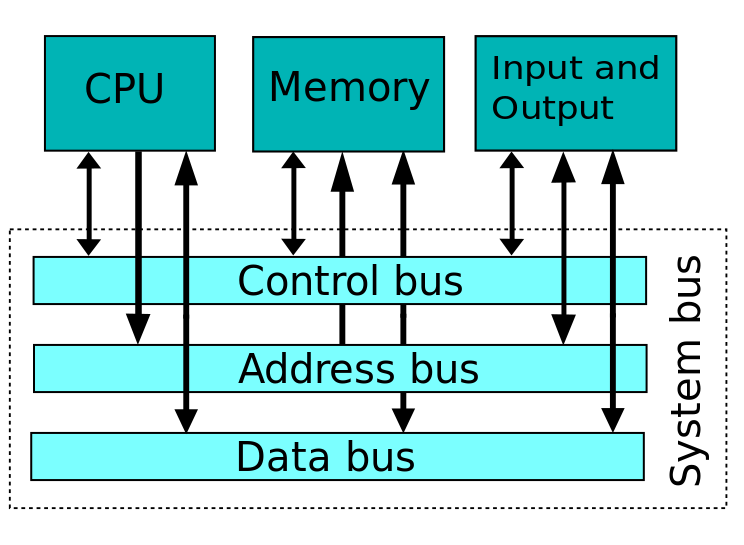
\includegraphics[scale=0.4]{fig/von_neuman}
	\caption{Von Neuman}
	\label{vn}
\end{figure}
\end{frame}

%%%
\begin{frame}[fragile]
\frametitle{Co znamená "počítačový program"?}
% obrazek
\begin{itemize} % vylepsit popis
	\item Pro (většinu) lidí jde o zdrojový kód
\begin{verbatim}
	...
	pokus\_file = open\_file("pokus.txt");
	content = read\_file(pokus\_file);
	close\_file(pokus\_file);
\end{verbatim}
	\item Pro počítač jde o strojový kód
\begin{verbatim}
	...
	0010 1101 0100 0010
	0110 1000 1111 0001
\end{verbatim}
	\item Mezistupněm je jazyk symbolických adres (asembler)
\begin{verbatim}
	...
	mov eax, 0
	cmp eax, 4
	jne eax\_neni\_rovno
\end{verbatim}
\end{itemize}
\end{frame}

%%%
\begin{frame}
\frametitle{Běh software na počítači}
% obrazek z wiki!!!!!!!!!!!!
Von Neumannova architektura
\begin{itemize} % vylepsit popis
	\item Procesor(y) zpracovává(-ají) instrukce
	\item Na jejich základě přistupuje procesor do paměti a I/O zařízení
	\item Všechny části jsou spojeny sběrnicemi
\end{itemize}
\end{frame}

%%%
\begin{frame}
\frametitle{Co je jádro OS?}
% obrazek z wiki
\begin{itemize} % vylepsit popis
	\item Vrstva SW mezi HW a uživatelskými programy
	\item Vytváří prostředí pro běh uživatelských programů
	\item Vytváří abstrakci neustále dostupného CPU
	\item Vytváří abstrakci dostupné lineární paměti (viz. virtuální paměť dále)
	\item Zpřístupňuje I/O zařízení uživatelských programům
\end{itemize}
\end{frame}

\begin{frame}
\frametitle{Co je jádro OS?}
\begin{figure}[h]
	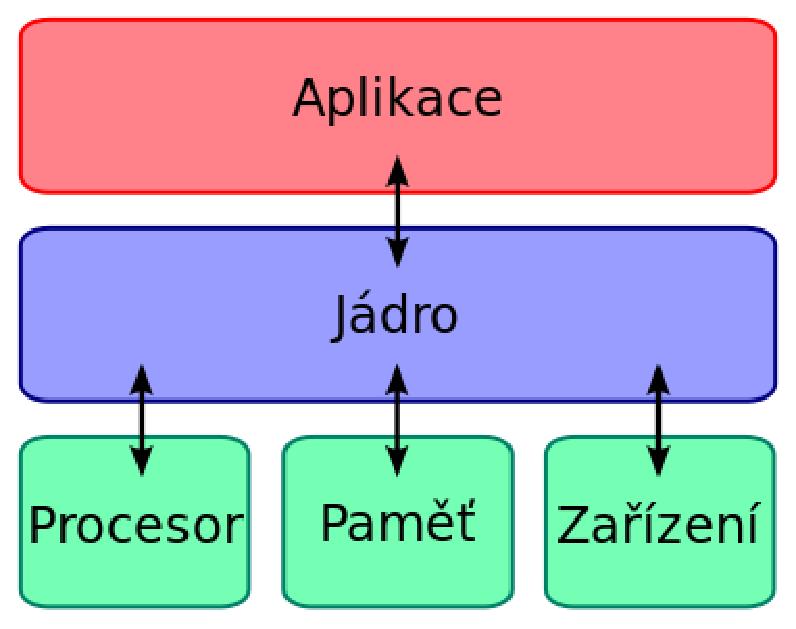
\includegraphics[scale=0.4]{fig/kernel}
	\caption{Kernel}
	\label{kern}
\end{figure}
\end{frame}

%%%
\begin{frame}
\frametitle{Rozhraní jádra}
% obrazek
\begin{itemize} % vylepsit popis
	\item systémové volání (read(), iotctl(), ...)
	\item socket (netlink, udp)
	\item procfs, sysfs, debugfs, ...
	\item ...
\end{itemize}
\end{frame}

%%%
\begin{frame}
\frametitle{userspace x kernelspace}
% obrazek
\begin{itemize} % vylepsit popis
	\item kernelspace - vše, co se děje v prostoru jádra operačního systému
	\item userspace - vše, co se NEděje v prostoru jádra operačního systému
\end{itemize}
\end{frame}

%%%
\begin{frame}[fragile]
\frametitle{Režimy činnosti procesoru}
% obrazek
\begin{itemize} % vylepsit popis
	\item HW ochrana systému
	\item Dva režimy - uživatelský (user mode) a privilegovaný (kernel mode)
\end{itemize}
\begin{itemize}
	\item Uživatelský - vykonává kód aplikace
	\item Privilegovaný - vykonává přístup k HW, do paměti
\end{itemize}
\begin{verbatim}
	buffer = read(openedfile);
	  ^---- volani C knihovny
	     ^---- volani systemoveho volani read()
		----------> prechod do privilegovaneho rezime
	        ^---- cteni z disku(cache)
\end{verbatim}
\end{frame}

%%%
\begin{frame}
\frametitle{Reprezentace procesu}
% obrazek
\begin{itemize} % vylepsit popis
	\item Proces ~ program (!)
	\item Proces má přiřazené process ID (PID)
	\item Může být tvořen více vlákny (rozdíl proces vs. vlákno)
	\item Jádro si musí stále pamatovat jeho
	\begin{itemize}
		\item stav
		\item otevřené soubory/zařízení
		\item úsek paměti, který používá
		\item otce/potomky (fork())
		\item statistiky o běhu
		\item a mnoho dalšího..
	\end{itemize}
\end{itemize}
\end{frame}

%%%
\begin{frame}
\frametitle{Správa a plánování procesů}
% obrazek
\begin{itemize} % vylepsit popis
	\item Toto přidělování řídí \textit{plánovač}
	\item Plánování je preemptivní nebo nepreemptivní
	\item Procesům jsou jádrem přidělovány časová kvanta procesoru (u
		preemptivního)
\end{itemize}
\begin{description}
	\item[preemptivní] CPU může být kdykoliv procesu odebrán
	\item[nepreemptivní] CPU může být procesu odebrán, až mu to proces dovolí
\end{description}
\end{frame}


%%%
\begin{frame}
\frametitle{Hierarchie procesů}
% obrazek
\begin{itemize} % vylepsit popis
	\item Lze zobrazit programem \texttt{pstree}
	\item Počáteční proces je proces s PID 0
	\item Potomci jsou dále tvoření pomocí volání funkce \texttt{fork()} uvnitř rodičovského procesu
	\item Pokud je dřív ukončen potomek, otcovský proces si přebírá jeho návratovou hodnotu (do té doby je zombie)
	\item Pokud je dřív ukončen rodič, potomek se stává potomkem procesu s PID 0
\end{itemize}
\end{frame}


%%%
\begin{frame}
\frametitle{Stavy procesu}
% obrazek !!!!!
\begin{itemize} % vylepsit popis
		\item běžící - running: běží na procesoru nebo je připraven k běhu ve frontě
		\item čekající - uninterruptible sleep: čeká typicky na dokončení I/O operace
		\item uspaný - interruptible sleep: čeká na dokončení události nebo uplynutí časovače
		\item zombie - ukončený proces, kterého si dosud jeho otec nepřevzal
\end{itemize}
Lze zobrazit například pomocí programu \texttt{htop}
\end{frame}


%%%
\begin{frame}
\frametitle{Synchronizace mezi procesy}
% obrazek
\begin{itemize} % vylepsit popis
	\item Na jednom systému může běžet *mnoho* procesů současně
	\item Procesy mají k dispozici omezený počet "zdrojů" (paměť, úložný prostor)
	\item Dochází k "souboji" procesů o zdroje
	\item Synchronizace pomocí zámků, mutexů nebo semaforů
	\item Existují následující scénáře, ke kterým by nemělo docházet:
\end{itemize}
\begin{description}
	\item [deadlock] - Procesy si navzájem blokují závislé zdroje => nikdo nemůže pokračovat
	\item [vyhladovění] - Proces je stále předbíhán procesy s vyšší prioritou
\end{description}
\end{frame}

%%%
\begin{frame}
\frametitle{Deadlock}
\begin{figure}[h]
	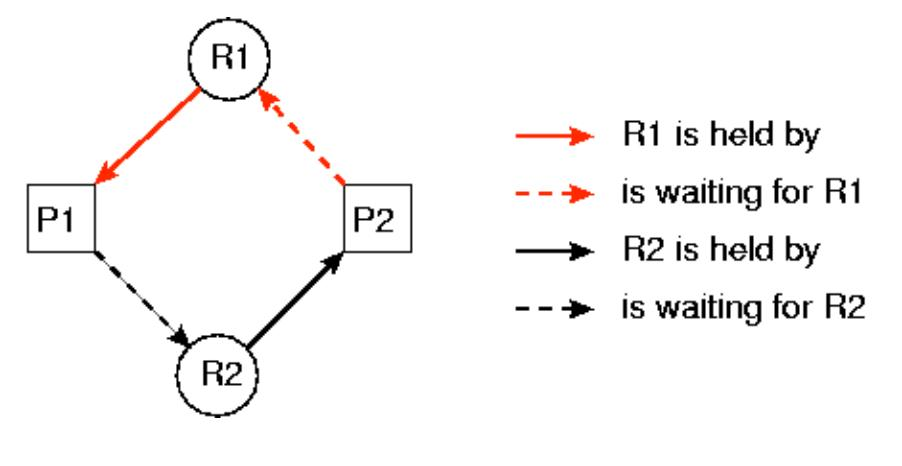
\includegraphics[scale=0.4]{fig/deadlock}
	\caption{Deadlock}
	\label{dd}
\end{figure}
\end{frame}

%%%
\begin{frame}
\frametitle{Vyhladovění}
\end{frame}

%%%
\begin{frame}
\frametitle{Správa paměti}
% obrazek
\begin{itemize} % vylepsit popis
	\item Procesy potřebují ke svému běhu vždy paměť
	\item Jádro operačního systému ji musí jednoduše poskytnout
	\item Problémy: mnoho procesů, omezená velikost paměti, nutnost izolace paměti mezi procesy
	\item Jedno z řešení = virtuální paměť
\end{itemize}
\end{frame}

%%%
\begin{frame}
\frametitle{Paměťová hierarchie}
\begin{itemize}
\item Uspořádání paměťových úložišť:
	\begin{itemize}
		\item Vzestupně podle kapacity
		\item Sestupně podle rychlosti
	\end{itemize}
\item Data se pohybují oběma směry
\item Stupně:
	\begin{itemize}
	\item Registry procesoru
	\item Cache (L1, L2, L3)
	\item Hlavní paměť (RAM - Random Access Memory)
	\item Sekundární úložiště (disk, páska)
	\end{itemize}
\end{itemize}
\end{frame}

%%%
\begin{frame}
\frametitle{Paměťová hierarchie}
\begin{figure}[h]
	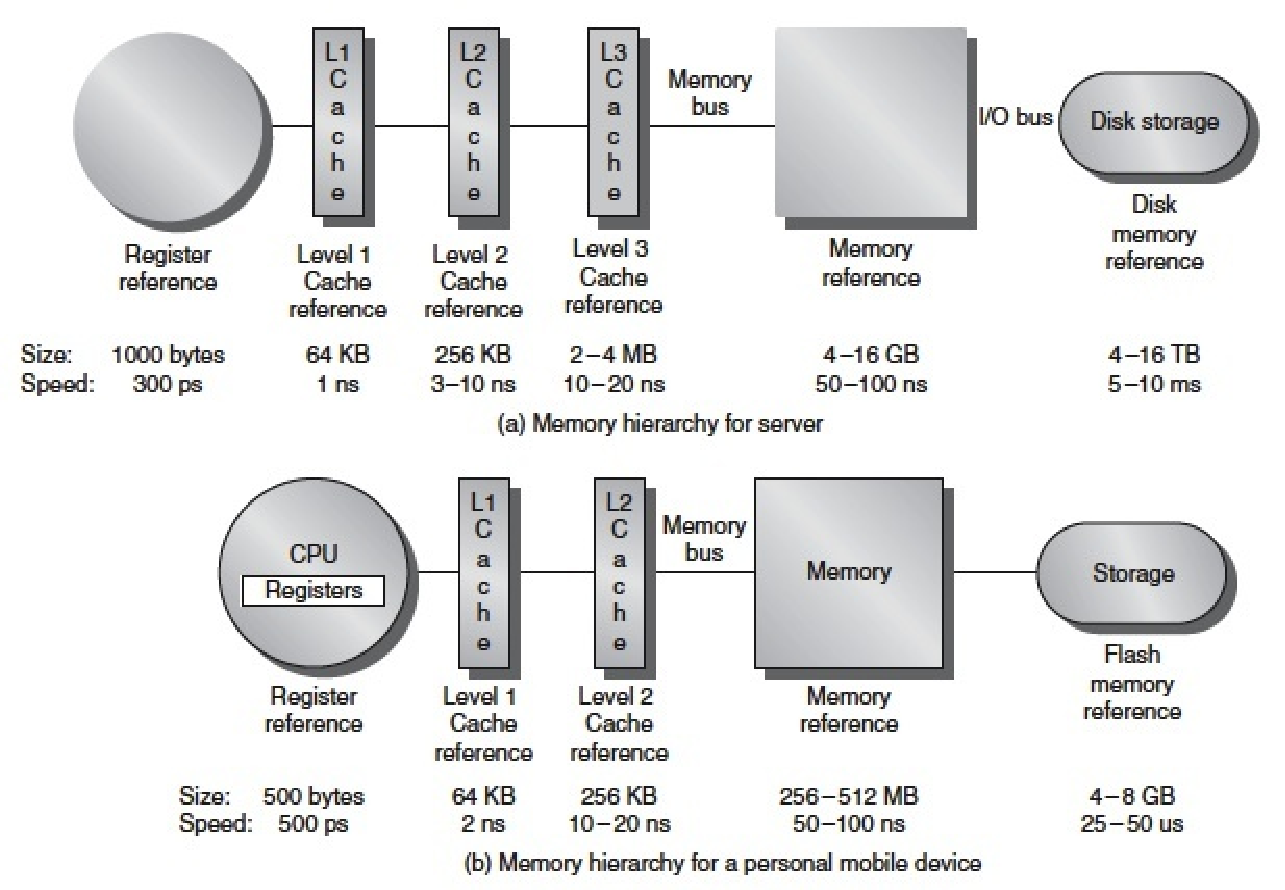
\includegraphics[width=\textwidth,keepaspectratio]{fig/hier}
	\caption{Paměťová hierarchie (zdroj: Hennessy, Patterson)}
	\label{hier}
\end{figure}
\end{frame}

%%%
 \begin{frame}
\frametitle{Stránkování}
\begin{itemize}
\item Na všech moderních OS je nejmenší použitelné množství paměti 1 stránka
\item Typicky 4kB, existují však i větší (viz. hugepages v Linuxu)
\item Z pohledu OS rozlišujeme dva typy stránek:
	\begin{itemize}
		\item Virtuální stránky - viditelné pro běžící procesy a tedy programátory
		\item Fyzické rámce - paměť v RAM
	\end{itemize}
\end{itemize}
\end{frame}

%%%
\begin{frame}
\frametitle{Virtuální paměť}
\begin{itemize}
\item Koncept řešící současný běh více procesů na jednom systému
\item Každý běžící proces má k dispozici 4GB adresového prostoru rozděleného na jednotlivé \textit{stránky}
\item Virtuální paměť řeší přiřazení fyzických rámců ke stránkám virtuálních (ne nutně 1:1 - u sdílených knihoven)
\item Adresa \texttt{0x89f92ad2} u procesu $1$ ukazuje do jiné buňky paměti než stejná adresa u procesu $2$
\end{itemize}
\end{frame}

%%%
%%%
 \begin{frame}
\frametitle{Tabulka stránek}
\begin{itemize}
\item Udržuje mapování virtuálních stránek na fyzické rámce pro \textbf{každý} běžící proces
\item Adresa je rozdělena na několik částí podle počtu stupňů TS a offset
\item Hledání v tabulce je časově náročné, existuje tedy malá cache TLB (Translation lookaside buffer), která obsahuje poslední úspěšné překlady mapování
\item Při přepnutí procesu je TLB vyprázdňována
\end{itemize}
\end{frame}

%%%%
\begin{frame}
\frametitle{Tabulka stránek}
\begin{figure}[h]
	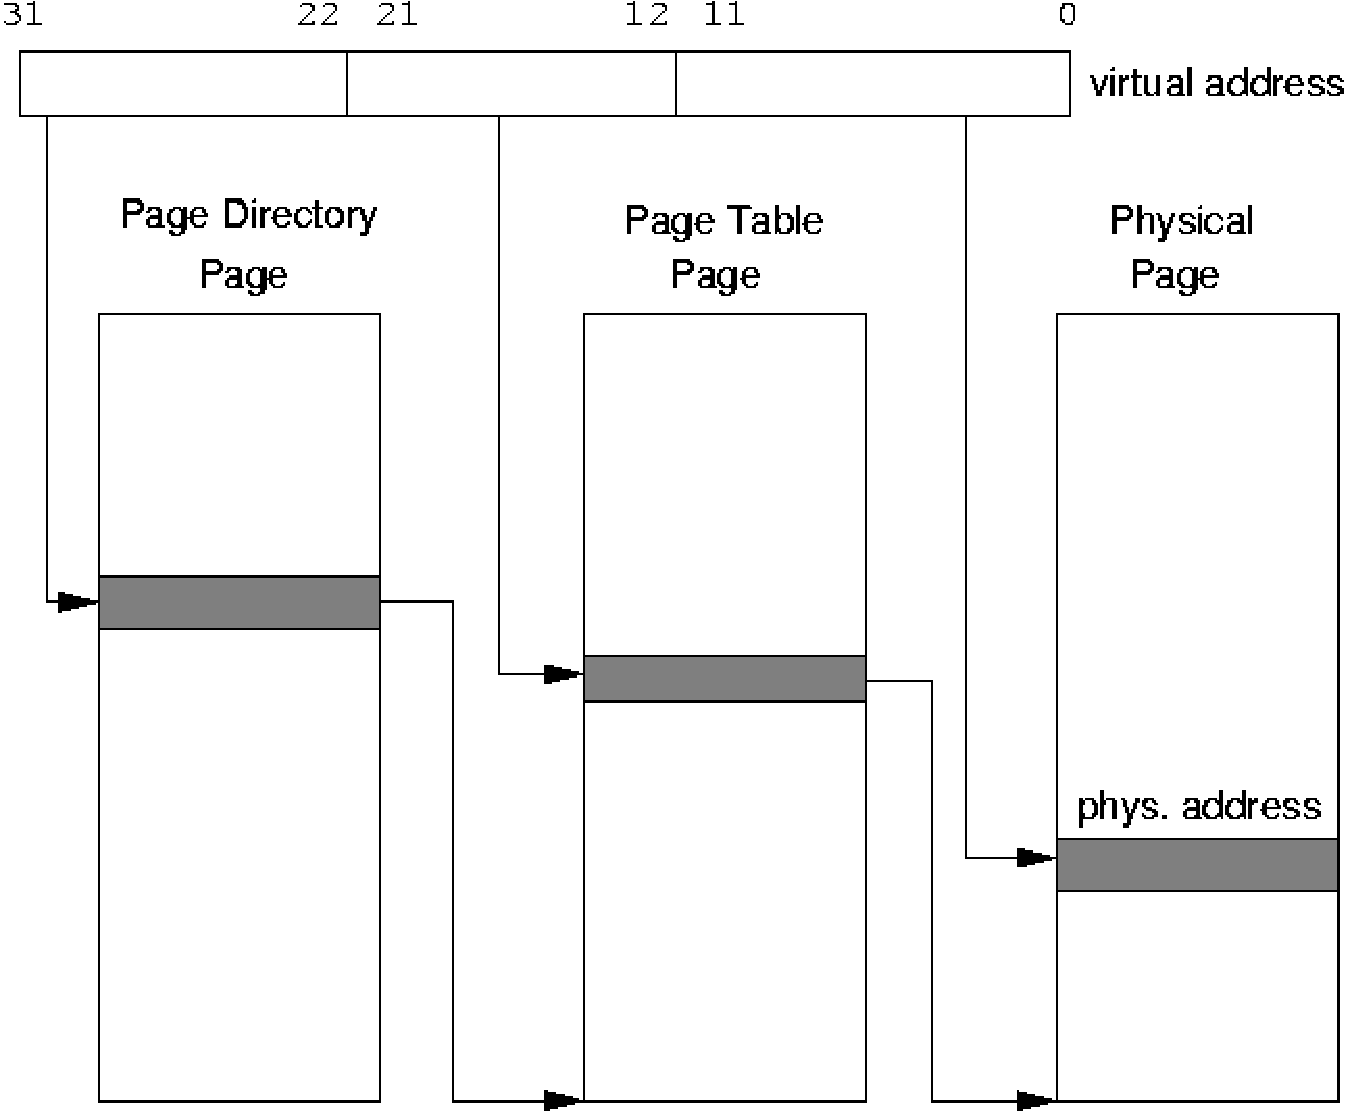
\includegraphics[scale=0.4]{fig/pgtable}
	\caption{Tabulka stránek}
	\label{vm}
\end{figure}
\end{frame}

%%%%
\begin{frame}
\frametitle{Překlad adres}
\begin{figure}[h]
	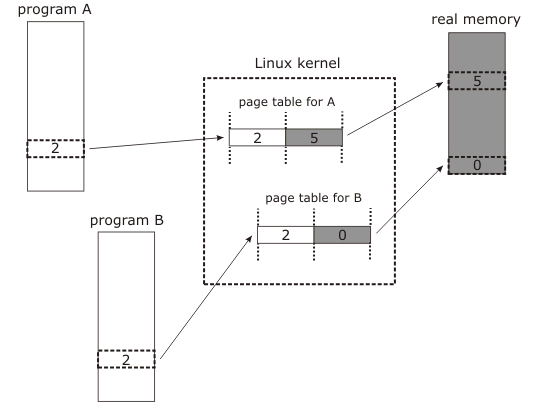
\includegraphics[width=\textwidth,keepaspectratio]{fig/vm}
	\caption{Překlad adres}
	\label{vm}
\end{figure}
\end{frame}

%%%
 \begin{frame}
\frametitle{Swapování stránek}
\begin{itemize}
\item Řeší záhadu proč může každý proces používat 4GB paměti i když je fyzicky nainstalováno méně RAM
\item Pokud je hlavní paměť RAM plná, jádro OS vybere nejméně potřebnou stránku a uloží ji na swap oddíl, typicky na sekundárním úložišti:
	\begin{itemize}
		\item v Linuxu obvykle samostatný diskový oddíl typu swap
		\item ve Windows stránkovací soubor viditelný přímo na disku
	\end{itemize}
\item Poté toto uvolněné místo ve fyzické paměti nahradí novou požadovanou stránkou
\item Při přístupu na stránku umístěnou ve swapu je stránka opět nahrána do hlavní paměti, kde opět vystřídá jinou, "nejméně" potřebnou, pokud není stále volné místo.
\item V designu paměťového podsystému je vždy velká snaha pomoci použití sofistikovaných algoritmů omezit použití swapu na minimum
\end{itemize}
\end{frame}

%%%
\begin{frame}
\frametitle{Načítání jádra při startu počítače}
% obrazek
\begin{enumerate} % vylepsit popis
	\item Zapnutí počítače
	\item Start BIOSu - kontrola HW, inicializace
	\item Načtení bootloaderu z MBR - 512 byte dlouhý úsek na začátku disku
	\item Běh bootloaderu, který vybere jádro a načte jej do paměti
\end{enumerate}
\end{frame}

%%%
\begin{frame}
\frametitle{Typy jader}
% obrazek
\begin{description} % vylepsit popis
	\item [mikrojádro] - implementuje pouze základní služby (paměť, procesy), zbytek implementován v uživatelském prostoru
	\item [monolitické] - vše implementováno uvnitř jádra - Linux
	\item [hybridní] - kompromis mezi dvěma přístup - Windows
\end{description}
\end{frame}

%%%
\begin{frame}
\frametitle{Vývoj linuxového jádra}
% obrazek LINUS
\begin{itemize} % vylepsit popis
	\item Finský programátor Linus Torvalds začal s vývojem v roce 1991
	\item Dosud hlavním šéfem a diktátorem vývoje
	\item První verze jádra měla ~ 10 000 řádků
	\item Linuxový kernel má v současné době přes 15 000 000 řádků
\end{itemize}
\end{frame}

\begin{frame}
\frametitle{Linus Torvalds}
\begin{figure}[h]
	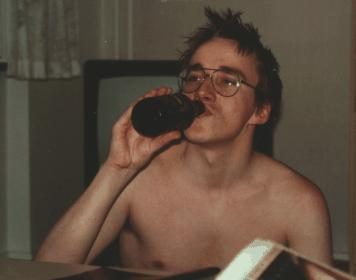
\includegraphics[scale=0.6]{fig/linus-torvalds-beer}
	\caption{Linus Torvalds}
	\label{linus}
\end{figure}
% obrazek
\end{frame}

%%%
\begin{frame}
\frametitle{Komunikace mezi vývojáři}
% obrazek
\begin{itemize} % vylepsit popis
	\item Změny se zasílají formou patchů - rozdílů v kódu
	\item Téměř výlučně je používán email + systém pro zprávu verzí git
	\item Linux Kernel Mailing List: https://lkml.org/
	\item Tisíce mailů denně od vývojářů z celého světa, ne úplně přátelské prostředí
	\item Až na výjimky velice vysoká úroveň kódu, který je přijat
\end{itemize}
\end{frame}


%%%
\begin{frame}[fragile]
\frametitle{Patch}
\begin{itemize}
\item Změna řádků v kódu
\item Hlavní způsob komunikace v OSS komunitě
\item ukázka
\end{itemize}
\end{frame}

%%%


%%%
 \begin{frame}
\frametitle{Literatura}
\begin{itemize}
\item \url{http://www.kernel.org/} 
\end{itemize}
\end{frame}


\end{document}
